%\VignetteIndexEntry{4. Journal of Statistical Software Article}
%\VignetteEngine{Sweave}
\documentclass[article]{jss}
\usepackage{thumbpdf} 
\graphicspath{{Figures/}}

\newcommand{\xmin}{x_{\min}}
\usepackage{amsmath}
\usepackage{microtype}
\usepackage[utf8]{inputenc} 
\usepackage{algorithm}

\author{Colin S. Gillespie\\Newcastle University}
\Plainauthor{Colin S. Gillespie}

\title{Fitting Heavy Tailed Distributions: The \pkg{poweRlaw} Package}
\Plaintitle{Fitting Heavy Tailed Distributions: The poweRlaw Package} 
\Shorttitle{\pkg{poweRlaw}: Fitting Heavy Tailed Distributions}

\Abstract{
  Over the last few years, the power law distribution has been used as
  the data generating mechanism in many disparate fields. However, at
  times the techniques used to fit the power law distribution have
  been inappropriate.  This paper describes the \pkg{poweRlaw}
  \proglang{R} package, which makes fitting power laws and other
  heavy-tailed distributions straightforward. This package contains \proglang{R}
  functions for fitting, comparing and visualizing heavy tailed
  distributions. Overall, it provides a principled approach to power
  law fitting.
} 

\Keywords{power laws, heavy tailed, fitting, estimation, \proglang{R}, Zipf, Pareto}
\Plainkeywords{power laws, heavy tailed, fitting, estimation, R, Zipf, Pareto}
 
\Volume{61}
\Issue{10}
\Month{October}
\Year{2014}
\Submitdate{2013-06-10}
\Acceptdate{2014-05-28}

\Address{
  Colin S. Gillespie \\
  School of Mathematics \& Statistics\\
  Newcastle University\\
  Newcastle upon Tyne\\
  NE1 7RU, United Kingdom\\
  E-mail: \email{colin.gillespie@newcastle.ac.uk}\\
  URL: \url{http://www.mas.ncl.ac.uk/~ncsg3/}
}

\usepackage{Sweave}
\begin{document}

\section{Introduction}\label{S1}

The nineteenth century Italian economist, Vilfredo Pareto, observed that many
processes do not follow the Gaussian distribution. This observation leads to the
so-called 80/20 rule, that is:
\begin{quote}
  \textit{80\% of all effects results from 20\% of all causes.}
\end{quote}
This rule has been used to describe a wide variety of phenomena. For
example, 20\% of employees of any business are responsible for 80\% of
productive output or 20\% of all people own 80\% of all wealth. By the
middle of the twentieth century, examples of these heavy tailed
distributions had been used to describe the number of papers published
by scientists, sizes of cities and word frequency (see
\citealt{Keller2005} for references).

In a similar vein, in 1999 two ground-breaking papers were published in
Science and Nature \citep{Barabasi1999,Albert1999}. In the first, the key result
was that the distribution of hyper-links in the World Wide Web seemed to follow
a power law distribution. Essentially, the connectivity of web pages, $k$,
decreased with rate $k^{\alpha}$. This suggested a large connection variance,
with a small number of large key nodes. The second paper presented a model that
could generate these networks and coined the phrase \textit{scale-free}. This
phrase implicitly linked these networks to the physics of phase transitions.

Since these two landmark papers, there has been an explosion in supposed
scale-free phenomena (see \cite{Clauset2009} for a recent overview). Particular
examples include
\begin{itemize}
\item the occurrence of unique words in the novel \textit{Moby Dick} by Herman
  Melville \citep{Newman2005}, Figure~\ref{F1}a;
\item casualty numbers in armed conflicts \citep{Bohorquez2009, Friedman2013}, Figure~\ref{F1}b;
\item comparing manually curated databases with automatically curated biological
  databases \citep{Bell2012}, Figure~\ref{F1}c.
\end{itemize}
Recently, this apparent ubiquity of power laws in a wide range of disparate
disciplines was questioned by \cite{Stumpf2012}. The authors point out that many
``observed'' power law relationships are highly suspect. In particular,
estimating the power law exponent on a log-log plot, whilst appealing, is a very
poor technique for fitting these types of models. Instead, a systematic,
principled and statistical rigorous approach should be applied (see
\citealt{Goldstein2004}).

In this paper we describe the \proglang{R} \citep{RCoreTeam2013} package
\pkg{poweRlaw} \citep{poweRlaw}. This package enables power laws and other heavy
tailed distributions, to be fitted in a straightforward manner. In particular,
the package provides an easy to use interface to the techniques proposed by
\cite{Clauset2009}. Functions are provided for plotting, comparing distributions
and estimating parameter uncertainty.

\begin{figure}[t] 
  \centering
  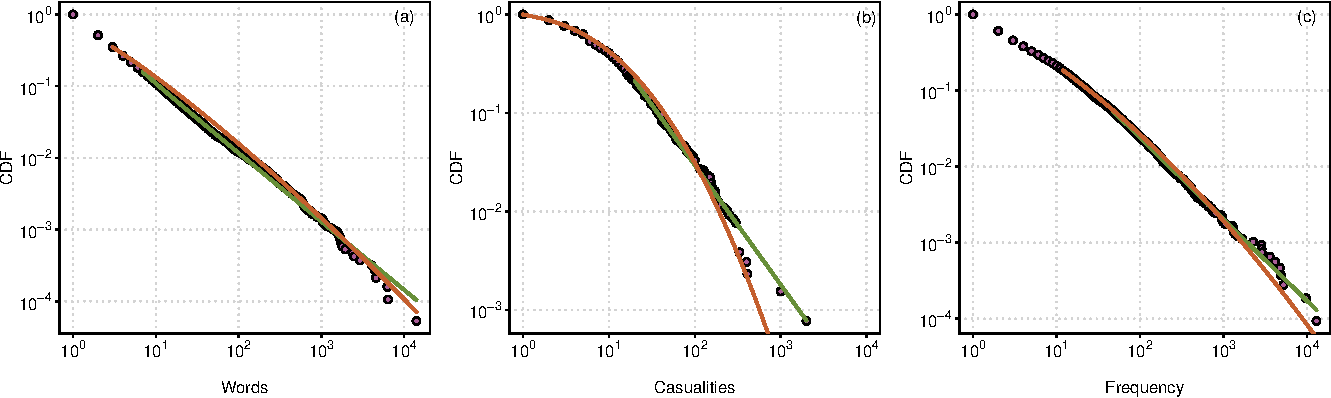
\includegraphics[width=\textwidth, trim = 0 0 0 0, clip]{figure1.pdf}
   \vspace*{-0.5cm}
 \caption{The cumulative distribution functions (CDFs) and their maximum
    likelihood power law (green) and log normal (orange) fit.  (a):
    Unique words in the novel Moby Dick. (b): Native American
    Casualities in the American Indian War. (c): Word frequency in the
    Swiss-Prot database (version 9). Further details of the data sets
    are given in Section~\ref{S1}.\label{F1}}
\end{figure}


At the most basic level, there are two types of power law
distributions: discrete and continuous. The continuous version has
probability density function (PDF)
\begin{equation}
p(x) = \frac{\alpha-1}{\xmin} \left(\frac{x}{\xmin}\right)^{-\alpha},
\end{equation}
where $\alpha >1$ and $\xmin >0$. While the discrete case has probability mass
function (PMF)
\begin{equation}
\Prob(X=x) = \frac{x^{-\alpha}}{\zeta(\alpha, \xmin)},
\end{equation}
where
\begin{equation}
\zeta(\alpha, \xmin) = \sum_{n=0}^{\infty} (n + \xmin)^{-\alpha}
\end{equation}
is the generalized zeta function \citep{Abramowitz1970}\footnote{The
  \pkg{poweRlaw} package uses the zeta function from the \pkg{VGAM} package to
  perform this calculation (see \citealt{Yee2010}).}. When $\xmin=1$,
$\zeta(\alpha, 1)$ is the standard zeta function. The cumulative density
functions have a relatively simple structure. For the continuous version we have
\begin{equation}
\Prob(X\le x) = 1-\left(\frac{x}{\xmin}\right)^{-\alpha + 1},
\end{equation}
whilst for the discrete version we have
\begin{equation}
\Prob(X \le x) = \frac{\zeta(\alpha, x)}{\zeta(\alpha, \xmin)} \;.
\end{equation}
The moments of the power law distribution are particularly interesting. For the
continuous power law we have
\[
\E[X^m] = \int_{\xmin}^{\infty} x^m p(x)\, dx = \frac{\alpha - 1}{\alpha - 1 -m}
\xmin^m \;.
\]
So when 
\begin{itemize}
\item $1< \alpha \le 2$, all moments diverge, i.e., $\E[X] = \infty$;
\item $2 < \alpha \le 3$, all second and higher-order moments diverge,
  i.e., $\E[X^2] = \infty$;
\item $3 < \alpha \le m+1$, all $m$ and higher-order moments diverge,
  i.e., $\E[X^m] = \infty$.
\end{itemize}

\subsection{Fitting heavy tailed distributions}\label{2.2}

To estimate the scaling parameter $\alpha$ is relatively
straightforward.  The maximum likelihood estimator (MLE) for the
continuous power law is
\begin{equation}\label{6}
  \hat \alpha = 1 + n \left[\sum_{i=1}^n \ln \frac{x_i}{\xmin}\right]^{-1},
\end{equation}
where $x_i$ are the observed data values and $x_i \ge \xmin$
\citep{Muniruzzaman1957}. The discrete MLE of $\hat \alpha$ is not available,
instead we use the approximation
\begin{equation}\label{7}
\hat \alpha \simeq 1 + n \left[\sum_{i=1}^n \ln \frac{x_i}{\xmin - 0.5}\right]^{-1} \;.
\end{equation}
The discrete MLE approximation is
identical to the exact continuous MLE, except for the additional $0.5$ in the
denominator (see \cite{Clauset2009} for a complete derivation). 

When calculating the MLE for $\alpha$, we \textit{condition} on a particular
value of $\xmin$. When power laws are used in practice, it is usually argued
that only the tails of the distribution follow a power law, and so $\xmin$ must
be estimated. However as $\xmin$ increases, the amount of data \textit{discarded}
also increases. So it clear that some care must be taken when choosing this
parameter.

The most common approach used to estimate $\xmin$ is from a visual inspection of
the data on a log-log plot. Clearly, this is highly subjective and error prone.
Instead, \cite{Clauset2009} recommend estimating the lower threshold using a
Kolmogorov-Smirnov approach. This statistic is simply the maximum distance
between the data and fitted model CDFs
\begin{equation}\label{8}
  D = \max_{x \ge \xmin} \vert S(x) - P(x) \vert,
\end{equation}
where $S(x)$ and $P(x)$ are the CDFs of the data and model respectively (for $x
\ge \xmin$). The estimate of $\xmin$ is the value of $\xmin$ that minimizes $D$.
This approach is completely general and can be used in conjunction with other
distributions.

\begin{algorithm}[t]
  \caption{Estimating the uncertainty in $\xmin$ \citep{Clauset2007}}\label{A1}
 \begin{tabular}{@{}ll@{}}
   {\small 1:} & Set $N$ equal to the number of values in the original data set. \\
   {\small 2:} & \textbf{for} \code{i} in \code{1:B}:\\
   {\small 3:} & $\quad$ Sample $N$ values (with replacement) from the original data set. \\
   {\small 4:} & $\quad$ Estimate $\xmin$ and $\alpha$ using the Kolmogorov-Smirnov statistic.\\
   {\small 5:} & \textbf{end for} \\
  \end{tabular}
\end{algorithm}

\subsection{Parameter uncertainty}\label{2.3}

For a particular value of $\xmin$, the standard error of the MLE $\hat
\alpha$ can be calculated analytically. However, to account for the
additional uncertainty of $\xmin$ it is necessary to use a bootstrap
procedure \citep{Efron1993}. Essentially, we sample with replacement
from the original data set and then re-infer the parameters at each
step (see Algorithm~\ref{A1}). The bootstrapping algorithm can be
applied to any distribution and can run in parallel.

\subsection{Alternative distributions}

The techniques discussed in the preceding sections provide flexible methods for
estimating distribution parameters and the lower cut-off, $\xmin$. In this
section, we discuss methods for testing whether the underlying distribution
could plausibly have a power law form.

Since it is possible to fit a power law distribution to \textit{any}
data set, it is appropriate to test whether the observed data actually
follows a power law. A standard goodness-of-fit test is to use
bootstrapping to generate a $p$~value to quantify the plausibility of
the hypothesis. If the $p$~value is large, then any difference between
the empirical data and the model can be explained with statistical
fluctuations. If $p \simeq 0$, then the model does not provide a
plausible fit to the data and another distribution may be more
appropriate. When testing against the power law distribution the
hypotheses are:
\begin{align*}
H_0\!\!:& \text{ the power law distribution can not be ruled out;}\\
H_1\!\!:& \text{ the power law distribution can be ruled out.}
\end{align*}
The bootstrapping procedure is detailed in
Algorithm~\ref{A2}. Essentially, we perform a hypothesis test by
generating multiple data sets (with parameters $\xmin$ and $\alpha$)
and then ``re-inferring" the model parameters. However, this technique
does have computational issues. In particular, when the scaling
parameter $\alpha \le 2$, the first moment (i.e., $\E[X]$) is infinite
and so extremely large values frequently occur. Since generating
random numbers for the discrete power law distributions involves
partitioning the cumulative density this may make this approach
unsuitable.

\begin{algorithm}[t]
  \caption{Testing the power law hypothesis \citep{Clauset2009}}\label{A2}
  \begin{tabular}{@{}ll@{}}
    {\small 1:} & Calculate point estimates for $\xmin$ and the scaling parameter $\alpha$. \\
    {\small 2:} & Calculate the Kolmogorov-Smirnov statistic, $KS_d$, for the original data set.\\
    {\small 3:} & Set $n_1$ equal to the number of values below $\xmin$. \\
    {\small 4:} & Set $n_2 = n - n_1$ and $P = 0$.\\
    {\small 5:} & \textbf{for} \code{i} in \code{1:B}:\\
    {\small 6:} & $\quad$ Simulate $n_1$ values from a uniform distribution:
    $U(1, \xmin)$ and $n_2$ values  \\
    &$\qquad$  from a  power law distribution (with parameter $\alpha$).\\
    {\small 7:} & $\quad$ Calculate the associated Kolmogorov-Smirnov statistic, $KS_{sim}$.\\
    {\small 8:} & $\quad$ If $KS_d > KS_{sim}$, then $P = P + 1$.\\
    {\small 9:} & \textbf{end for} \\
    {\small 10:} & $P= P/B$.\\
  \end{tabular}
\end{algorithm}

An alternative  approach to assessing the power law model is a direct comparison with
another model. A standard technique is to use Vuong's test, which is a
likelihood ratio test for model selection using the Kullback-Leibler criterion.
The test statistic, $R$, is the ratio of the log likelihoods of the data between
the two competing models. The sign of $R$ indicates which model is
\textit{better}. Since the value of $R$ is subject to error, we use the method
proposed by \cite{Vuong1989}. See Appendix C in \cite{Clauset2009} for further
details.


%\clearpage

\section{Example: word frequency in Moby Dick}

This example investigates the frequency of occurrence of unique words in the
novel Moby Dick by Herman Melville \citep{Clauset2009,Newman2005}. The data can
be downloaded from
\url{http://tuvalu.santafe.edu/~aaronc/powerlaws/data.htm}
or directly loaded from the \pkg{poweRlaw} package 
\begin{Schunk}
\begin{Sinput}
R> library("poweRlaw")
R> data("moby")
\end{Sinput}
\end{Schunk}
This data set contains the frequency of 18855 words. The most
commonly occurring word occurred 14086 times.

\subsection{Fitting a discrete power law}

To fit a discrete power law, we first create a discrete power law
object using the \code{displ} constructor\footnote{\code{displ}:
  \textbf{dis}crete \textbf{p}ower \textbf{l}aw.}
\begin{Schunk}
\begin{Sinput}
R> pl_m <- displ$new(moby)
\end{Sinput}
\end{Schunk}
The object \code{pl\_m} is an \proglang{S}4 reference
object. Initially the lower cut-off, $\xmin$, is set to the smallest
$x$ value and the scaling parameter, $\alpha$, is set to \code{NULL}.
\begin{Schunk}
\begin{Sinput}
R> pl_m$getXmin()
\end{Sinput}
\begin{Soutput}
[1] 1
\end{Soutput}
\begin{Sinput}
R> pl_m$getPars()
\end{Sinput}
\begin{Soutput}
NULL
\end{Soutput}
\end{Schunk}
The object also has standard setters:
\begin{Schunk}
\begin{Sinput}
R> pl_m$setXmin(5)
R> pl_m$setPars(2)
\end{Sinput}
\end{Schunk}
For a given $\xmin$ value, we can estimate the corresponding $\alpha$
value using its MLE.
\begin{Schunk}
\begin{Sinput}
R> estimate_pars(pl_m)
\end{Sinput}
\begin{Soutput}
$pars
[1] 1.926

$value
[1] 14873

$counts
function gradient 
       5        5 

$convergence
[1] 0

$message
[1] "CONVERGENCE: REL_REDUCTION_OF_F <= FACTR*EPSMCH"

attr(,"class")
[1] "estimate_pars"
\end{Soutput}
\end{Schunk}
Alternatively, we can estimate the exponent using a parameter scan
\begin{Schunk}
\begin{Sinput}
R> estimate_pars(pl_m, pars=seq(1.5, 2.5, 0.01))
\end{Sinput}
\end{Schunk}
To estimate the lower bound $\xmin$, we use the Kolmogorov-Smirnov approach
described in Section~\ref{2.2}
\begin{Schunk}
\begin{Sinput}
R> (est_pl <- estimate_xmin(pl_m))
\end{Sinput}
\begin{Soutput}
$KS
[1] 0.008253

$xmin
[1] 7

$pars
[1] 1.953

attr(,"class")
[1] "estimate_xmin"
\end{Soutput}
\end{Schunk}
For the Moby Dick data set, the minimum is achieved when $\xmin=7$ and $D(7) =
0.00825$. Similar to the \texttt{estimate\_pars}
functions we can limit the search space using the \texttt{xmin} and
\texttt{pars} arguments.

To set the power law object to these optimal values, we just use the
\code{xmin} setter.
\begin{Schunk}
\begin{Sinput}
R> pl_m$setXmin(est_pl)
\end{Sinput}
\end{Schunk}
To allow the user to explore different distributions and model fits, all
distribution objects have generic plot methods. For example,
\begin{Schunk}
\begin{Sinput}
R> plot(pl_m)
\end{Sinput}
\end{Schunk}
creates a log-log plot of the data, while the \code{lines} function
\begin{Schunk}
\begin{Sinput}
R> lines(pl_m, col=2)
\end{Sinput}
\end{Schunk}
adds the fitted distribution (to get Figure~\ref{F1}a). When calling the
\code{plot} and \code{lines} function, the data plotted is 
invisibly returned, i.e.,
\begin{Schunk}
\begin{Sinput}
R> dd <- plot(pl_m)
R> head(dd, 3)
\end{Sinput}
\begin{Soutput}
  x      y
1 1 1.0000
2 2 0.5141
3 3 0.3505
\end{Soutput}
\end{Schunk}
This makes it straightforward to create graphics using other
\proglang{R} packages.

To fit other distributions, we follow a similar procedure. For
example, to fit the discrete log normal distribution, we begin by
creating a `\code{dislnorm}' object and estimating the
parameters\footnote{\code{dislnorm}: \textbf{dis}crete
  \textbf{l}og-\textbf{norm}al.}.
\begin{Schunk}
\begin{Sinput}
R> ln_m <- dislnorm$new(moby)
R> (est_ln <- estimate_xmin(ln_m))
\end{Sinput}
\end{Schunk}
Then we update the object
\begin{Schunk}
\begin{Sinput}
R> ln_m$setXmin(est_ln)
\end{Sinput}
\end{Schunk}
and add the corresponding line to the plot
\begin{Schunk}
\begin{Sinput}
R> lines(ln_m, col=2)
\end{Sinput}
\end{Schunk}
giving Figure~\ref{F1}a. 

Figure~\ref{F1} gives example data sets, with associated power law and log
normal fits. Plotting the data in this manner has two clear benefits. First, it
highlights how much data is being discarded when fitting $\xmin$. Second,
it provides an easy comparison with other distributions. 


\subsection{Parameter uncertainty}

\begin{figure}[t]
 \centering
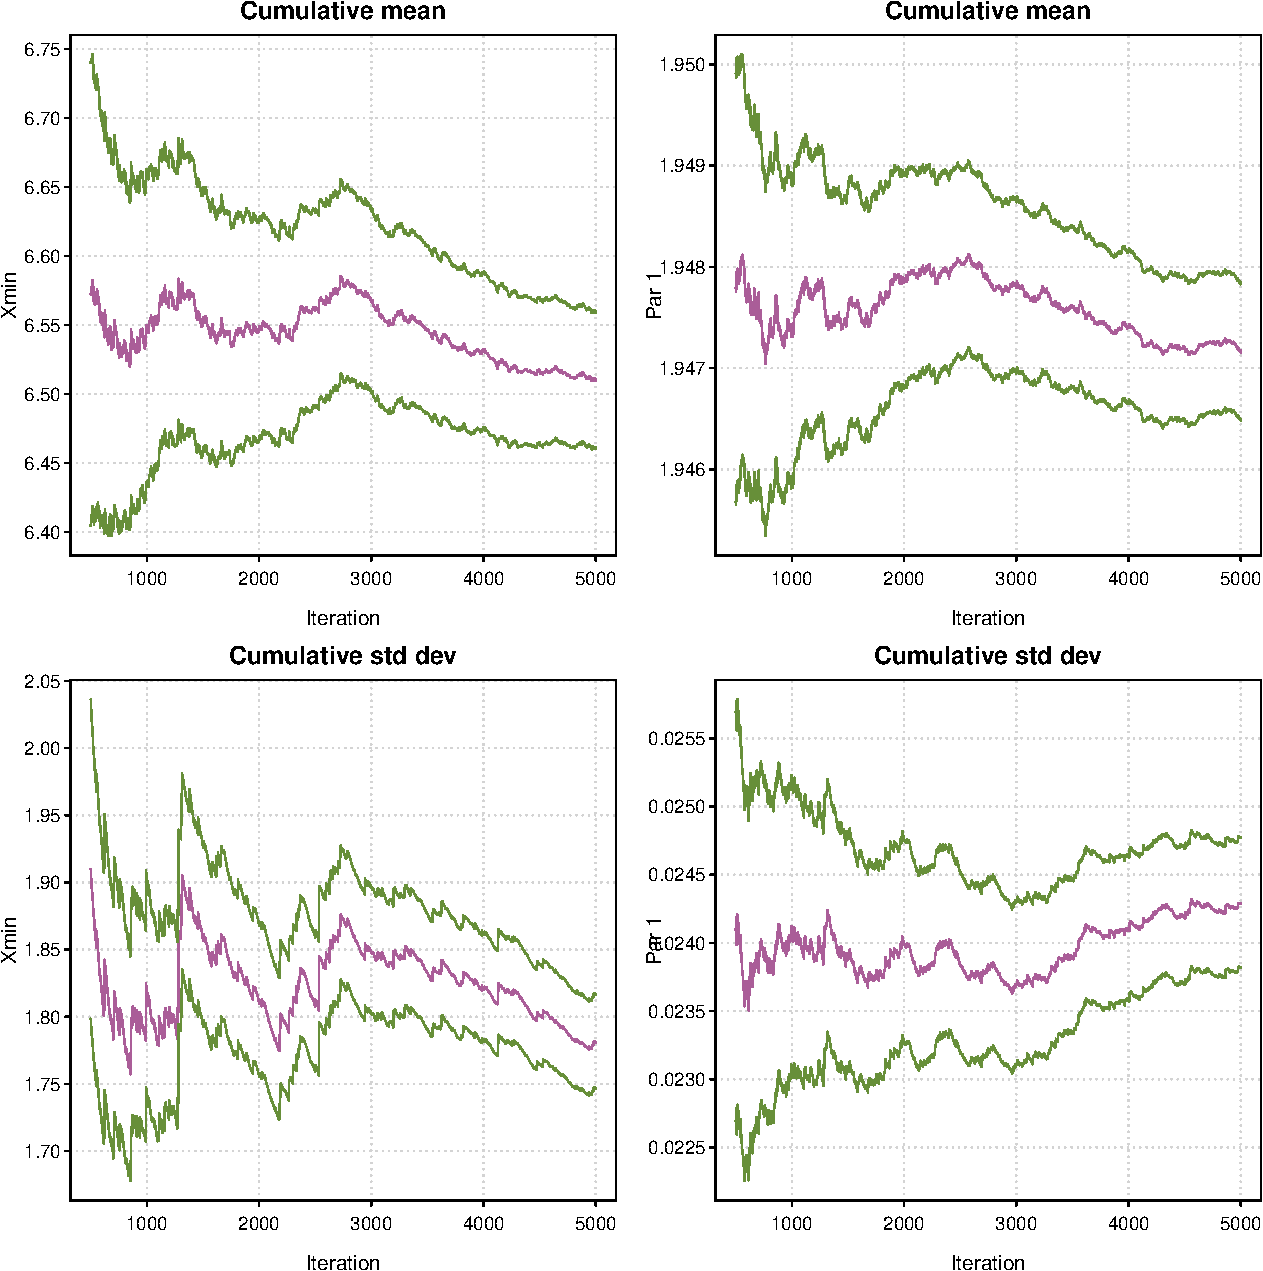
\includegraphics[width=0.7\textwidth]{figure2}
\caption{Results from the standard bootstrap procedure (for the power law model)
  using the Moby Dick data set: \mbox{\code{bootstrap(pl\_m)}}. The top row
  shows the sequential mean estimate of parameters $\xmin$ and $\alpha$. The
  bottom row shows the sequential estimate of standard deviation for each
  parameter. The dashed-green lines give approximate 95\% confidence intervals.
  After 5000 iterations, the standard deviation of $\xmin$ and $\alpha$ is
  estimated to be 1.9 and 0.02 respectively.}\label{F2}
\end{figure}                    %

To get a handle on the uncertainty in the parameter estimates, we use a
bootstrapping procedure, via the \code{bootstrap} function. This procedure can
be applied to \textbf{any} distribution object. Furthermore, the bootstrap
procedure can utilize multiple CPU cores to speed up inference using the base
package \pkg{parallel}. To generate five thousand bootstrap samples, using two
cores, we use the following command.
\begin{Schunk}
\begin{Sinput}
R> bs <- bootstrap(pl_m, no_of_sims=5000, threads=2)
\end{Sinput}
\end{Schunk}
By default the \code{bootstrap} function will use the MLE to infer the
parameter values and check all values of $\xmin$. When the $\xmin$
search space is large, then it is recommend that it is truncated.  For
example
\begin{Schunk}
\begin{Sinput}
R> bootstrap(pl_m, xmins=seq(2, 20, 2))
\end{Sinput}
\end{Schunk}
will only calculate the Kolmogorov-Smirnov statistics at values of $\xmin$ equal to
\[
2, 4, 6, \ldots, 20\;.
\]
A similar argument exists for the parameters.

The bootstrap function returns a `\code{bs\_xmin}' object. This object is a list
that consists of three components:
\begin{enumerate}
\item \code{gof}: the goodness-of-fit statistic obtained from the
  Kolmogorov-Smirnov test. This value should correspond to the value
  obtained from the \mbox{\code{estimate\_xmin}} function;
\item \code{bootstraps}: a data frame containing the results from the bootstrap procedure;
\item \code{sim\_time}: the average simulation time, in seconds, for a single bootstrap.
\end{enumerate}
The bootstrap results can be explored in a variety of ways. First we
can estimate the standard deviation of the parameter uncertainty,
i.e.,
\begin{Schunk}
\begin{Sinput}
R> sd(bs$bootstraps[,2])
\end{Sinput}
\begin{Soutput}
[1] 1.781
\end{Soutput}
\begin{Sinput}
R> sd(bs$bootstraps[,3])
\end{Sinput}
\begin{Soutput}
[1] 0.02429
\end{Soutput}
\end{Schunk}
Alternatively, we can visualize the results using the \code{plot}
method
\begin{Schunk}
\begin{Sinput}
R> plot(bs, trim=0.1)
\end{Sinput}
\end{Schunk}
to obtain Figure~\ref{F2}. The top row of graphics in Figure~\ref{F2}
give a sequential 95\% confidence interval for the mean estimate of
the parameters. The bottom row of graphics give a 95\% confidence
interval for the standard deviation of the parameters. The parameter
\code{trim} in the \code{plot} function controls the percentage of
samples displayed. When \code{trim=0}, all iterations are
displayed. When \code{trim=0.1}, we only display the final 90\% of
data.
\begin{figure}[t]
\centering 
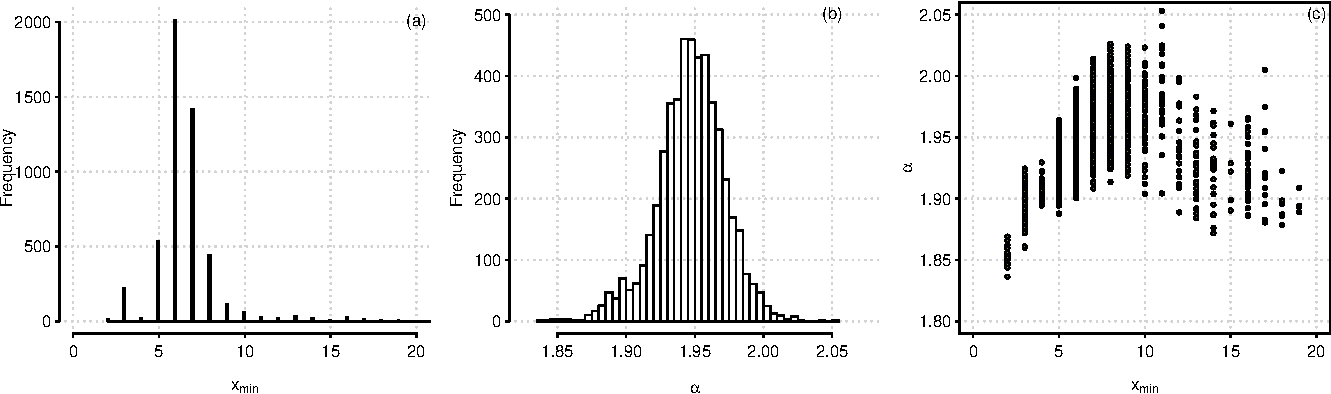
\includegraphics[width=\textwidth]{figure3}
  \vspace*{-0.5cm}
\caption{Characterizing uncertainty in parameter values using five
  thousand bootstraps.\newline
  (a) Histogram of $\xmin$ (standard deviation
  1.9). (b) Histogram of $\alpha$ (standard deviation 0.02). (c)
  Scatter-plot of the $\xmin$ against $\alpha$.\label{F3}}
\end{figure}

We can also construct histograms of the parameters
\begin{Schunk}
\begin{Sinput}
R> hist(bs$bootstraps[,2], breaks="fd")
R> hist(bs$bootstraps[,3], breaks="fd") 
\end{Sinput}
\end{Schunk}

to get Figures~\ref{F3}a \& b. A joint scatter plot is useful in highlighting
the strong dependency that often exists between the scaling parameter $\alpha$
and $\xmin$
\begin{Schunk}
\begin{Sinput}
R> plot(bs$bootstraps[,2], bs$bootstraps[,3])
\end{Sinput}
\end{Schunk}
and yields Figure~\ref{F3}c.

A similar bootstrap analysis can be obtained for the log normal distribution
\begin{Schunk}
\begin{Sinput}
R> bootstrap(ln_m)
\end{Sinput}
\end{Schunk}
In this case we would obtain uncertainty estimates for both of the log normal parameters.

\subsection{Comparison to other distributions}

The main thrust of \cite{Stumpf2012} is that many of the systems that are
characterized as having a power law distribution, could equally come from another
heavy tailed distribution. The \pkg{poweRlaw} package provides two methods for
testing the power law hypotheses.

\begin{figure}[t]
\centering 
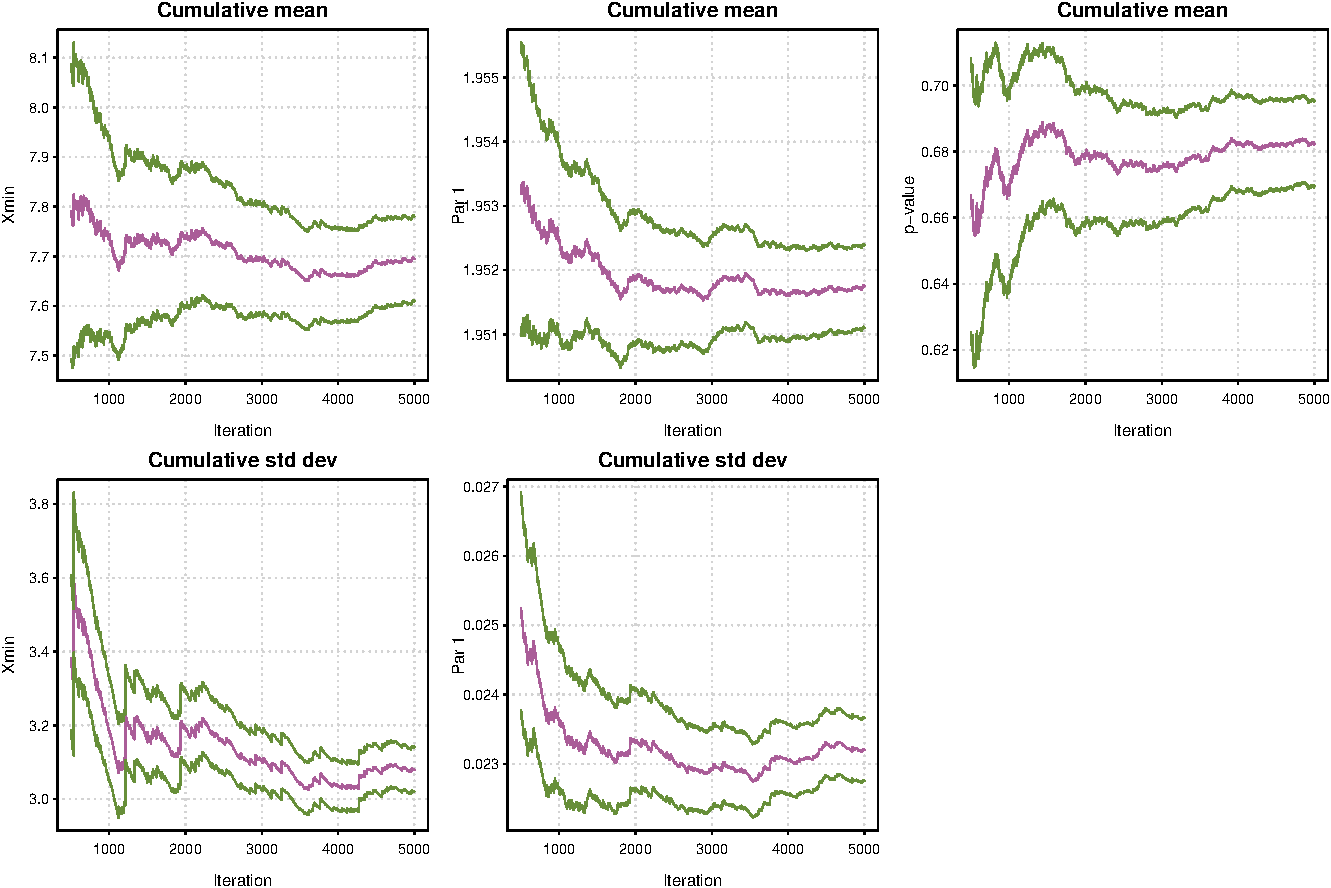
\includegraphics[width=\textwidth]{figure4}
 \vspace*{-0.5cm}
 \caption{Results from the bootstrap procedure for determining the plausibility
   of the power law hypothesis for the Moby Dick data set:
   \mbox{\code{bootstrap\_p(m\_pl)}}. The top row shows the sequential mean
   estimate of parameters $\xmin$, $\alpha$ and the $p$~value. The bottom row
   shows the sequential estimate of standard deviation for each parameter. The
   dashed-green lines give approximate 95\% confidence intervals. }\label{F4}
\end{figure}

The first method uses the bootstrapping technique described in Algorithm~\ref{A2}. This
is accessed using a similar interface as the standard bootstrap function.
\begin{Schunk}
\begin{Sinput}
R> bs_p <- bootstrap_p(pl_m)
\end{Sinput}
\end{Schunk}
%
Again this function can be run in parallel (using the \code{threads} argument) and
has the option to restrict the $\xmin$ search space. The output from the
\code{bootstrap\_p} function has very similar structure to the \code{bootstrap}
function. However, this function does return one additional element -- the
$p$~value for the hypothesis test:
\begin{align*}
H_0\!\!:& \text{ the power law distribution can not be ruled out;}\\
H_1\!\!:& \text{ the power law distribution can be ruled out.}
\end{align*}
In this particular example, we estimate $p=0.681$, i.e., the
underlying distribution for generating the Moby Dick data set could be
a power law distribution. Again, the output can be easily visualized with
\begin{Schunk}
\begin{Sinput}
R> plot(bs_p)
\end{Sinput}
\end{Schunk}
to obtain Figure~\ref{F4}. Notice that Figure~\ref{F4} has an additional plot
for the $p$~value. This enables the user to assess the accuracy of the estimated
$p$~value.

The second method is to directly compare two distributions using a likelihood
ratio test. For this test, both distributions must use the same $\xmin$ value.
For example, to compare the power law model to the log normal, we first the set
threshold to be the same as the power law model.
\begin{Schunk}
\begin{Sinput}
R> ln_m <- dislnorm$new(moby)
R> ln_m$setXmin(7)
\end{Sinput}
\end{Schunk}
Next we estimate the parameters (conditional on $\xmin=7$)
\begin{Schunk}
\begin{Sinput}
R> est <- estimate_pars(ln_m) 
\end{Sinput}
\end{Schunk}
and update the model
\begin{Schunk}
\begin{Sinput}
R> ln_m$setPars(est)
\end{Sinput}
\end{Schunk}
Then we can use Vuong's method to compare models.
\begin{Schunk}
\begin{Sinput}
R> comp <- compare_distributions(pl_m, ln_m)
\end{Sinput}
\end{Schunk}

The object \code{comp} object contains Vuong's test statistic, $p$~value and the
ratio of the log likelihoods. For this particular comparison, we have
$p=0.682$ which relates to the hypotheses
\begin{align*}
H_0\!\!:& \text{ both distributions are equally far from the true distribution;}\\
H_1\!\!:& \text{ one of the test distributions is closer to the true distribution.}
\end{align*}
Hence, we cannot reject $H_0$ and it is not possible to determine
which is the best fitting model.

\section{Package overview }

In the previous example we created a `\code{displ}' object
\begin{Schunk}
\begin{Sinput}
R> pl_m <- displ$new(moby)
\end{Sinput}
\end{Schunk}
to represent the discrete power law distribution. This particular object has
class `\code{displ}' and also inherits the `\code{discrete\_distribution}' class.
Other available distributions are given in Table~\ref{T2}. 
\begin{table}[t!]
   \centering
  \begin{tabular}{@{} llc @{}}
    \hline
    Distribution & Class name & \# of parameters \\
    \hline
    Discrete power law & `\code{displ}' & 1 \\
    Discrete log normal & `\code{dislnorm}' & 2 \\
    Discrete exponential & `\code{disexp}' & 1 \\
    Poisson & `\code{dispois}' & 1 \\ \hline
    Continuous power law & `\code{conpl}' & 1 \\
    Continuous log normal & `\code{conlnorm}' & 2 \\
    Exponential & `\code{conexp}' & 1 \\
    \hline
  \end{tabular}
  \caption{Available distributions in the \pkg{poweRlaw} package. Each class
    also inherits either the `\code{discrete\_distribution}' or `\code{ctn\_distribution}' class.}\label{T2}
\end{table}

\begin{figure}[t]
\centering 
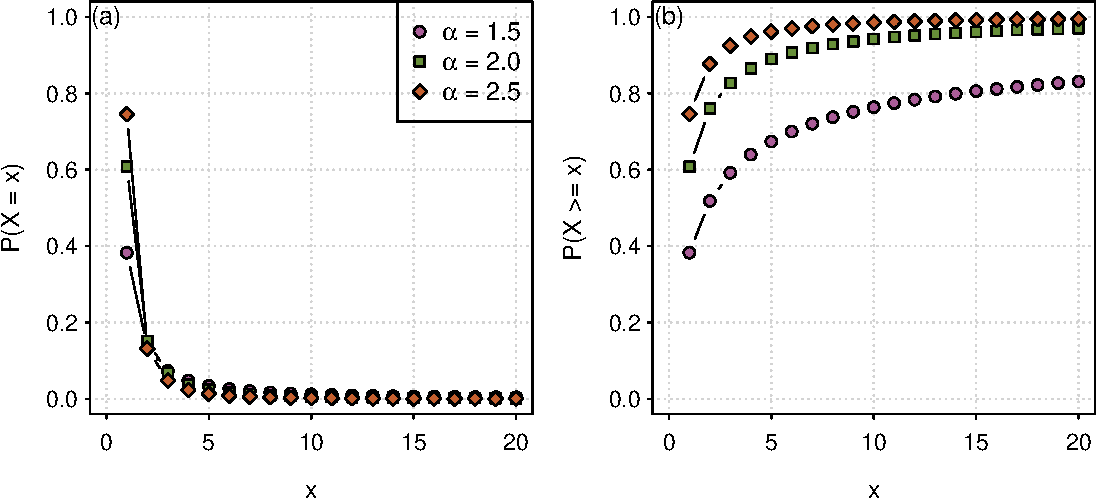
\includegraphics[width=0.8\textwidth]{figure5}
\caption{The (a) probability mass function and (b) probability distribution
  function for the discrete power law, where $\xmin=1$ and $\alpha$ as indicated.}\label{F5}
\end{figure}

The classes given in Table~\ref{T2} are \proglang{S}4 reference
classes\footnote{See \code{\mbox{?setRefClass}} for further details on
  reference classes.}. Each `\code{distribution}' object has four fields:
\begin{itemize}
\item \code{dat}: the data set;
\item \code{xmin}: the lower cut-off $\xmin$;
\item \code{pars}: a vector of parameter values;
\item \code{internal}: a list of values used in different numerical
  procedures. This will differ between distribution objects. In general, the
  user will not interact with the \code{internal} field.
\end{itemize}
Using this particular object orientated framework has three distinct benefits. 
\begin{enumerate}
\item After fitting a single distribution, fitting all other distributions
  follows an almost identical route.
\item It is straightforward to add new distributions to the package.
\item The \code{internal} field allows efficient caching of data structures when
  updating the \code{xmin} and \code{pars} fields. In particular, when the data is
  first loaded, efficient vector operations can be carried out and used as a
  look-up table, i.e., taking $\log$'s of the data.
\end{enumerate}
Distribution objects have a number of methods available (see Table~\ref{T3}).
All \code{dist\_*} methods depend on the \textit{type} of distribution. For
example, to plot the probability mass function of the discrete power law
distribution, we first create a discrete power law object
\begin{Schunk}
\begin{Sinput}
R> m <- displ$new()
R> m$setXmin(1)
\end{Sinput}
\end{Schunk}
then use the \code{dist\_pdf} function to obtain the probabilities for particular
parameter values
\begin{Schunk}
\begin{Sinput}
R> x <- 1:20
R> m$setPars(1.5)
R> plot(x, dist_pdf(m, x), type="b")
R> m$setPars(2.0)
R> lines(x, dist_pdf(m, x), type="b")
R> m$setPars(2.5)
R> lines(x, dist_pdf(m, x), type="b")
\end{Sinput}
\end{Schunk}
This gives Figure~\ref{F5}a. Likewise, to obtain the CDF we use the
\code{dist\_cdf} function, i.e.,
\begin{Schunk}
\begin{Sinput}
R> plot(x, dist_cdf(m, x), type="b")
\end{Sinput}
\end{Schunk}
to obtain Figure~\ref{F5}b.

The other methods, \code{estimate\_*} and \code{bootstrap\_*}, work
with general distribution objects (although internally they use
\code{dist\_*} methods). See the associated help files for further
details.
\begin{table}[t!]
  \centering
  \begin{tabular}{@{} lp{12cm} @{}}
    \hline
    Method name & Description \\
    \hline
    \code{dist\_cdf} & Cumulative density/mass function (CDF)\\
    \code{dist\_pdf} & Probability density/mass function (PDF)\\
    \code{dist\_rand}& Random number generator\\
    \code{dist\_data\_cdf} & Data CDF \\
    \code{dist\_ll} & Log likelihood\\ \hline
    \code{estimate\_xmin} & Point estimates of the cut-off point and parameter values\\
    \code{estimate\_pars} & Point estimates of the parameters (conditional on the current $\xmin$ value)\\ \hline
    \code{bootstrap} & Bootstrap procedure (uncertainty in $\xmin$)\\
    \code{bootstrap\_p} & Bootstrap procedure to test whether we have a power law\\
    \hline
  \end{tabular}
  \caption{A list of methods available for `\code{distribution}' objects. These methods do not change the object states.}\label{T3}
\end{table}

\section{Conclusion}

In recent years an over-enthusiastic fitting of power laws to a wide
variety of systems has resulted in the inevitable (and needed) call
for caution.  \cite{Stumpf2012} correctly highlight that many supposed
power law relationships are at best dubious and some obviously
false. These problems in determining the underlying distribution of
these mechanisms can (in some part) be attributed to the lack of
available and easy to use software packages for fitting heavy tailed
distributions. The \pkg{poweRlaw} package aims to solve this
problem. By providing an easy to use and consistent interface,
researchers can now fit, and more importantly, compare a variety of
truncated distributions fitted to their data set.

\subsection*{Acknowledgements}

The author gratefully acknowledges Aaron Clauset and Jeff Friedman for their
constructive comments on the manuscript and discussions on the implementation of
the methodology.

\bibliography{v61i10}


\end{document}
